\documentclass{article}
\usepackage[dblblindworkshop]{neurips_2026}
\workshoptitle{AIMO Interpretability Challenge}
\usepackage[utf8]{inputenc}
\usepackage[T1]{fontenc}
\usepackage{hyperref}
\usepackage{url}
\usepackage{booktabs}
\usepackage{amsfonts}
\usepackage{nicefrac}
\usepackage{microtype}
\usepackage{xcolor}
\usepackage{graphicx}
\usepackage{array}
\hypersetup{pdftitle={Robustness labels follow the problem: six model signals fail on unseen problems, and a text-length control matches the kit baseline},pdfauthor={},pdfcreator={},pdfproducer={}}
\newcolumntype{R}[1]{>{\raggedleft\arraybackslash}p{#1}}
\providecommand{\tightlist}{\setlength{\itemsep}{0pt}\setlength{\parskip}{0pt}}
\title{Robustness labels follow the problem: six model signals fail on unseen problems, and a text-length control matches the kit baseline}
\author{}
\begin{document}
\maketitle
\noindent\emph{Technical report for the AIMO Interpretability Challenge writeup awards. Negative result. Tracks: Main and Small Models.}

\begin{abstract}

In the organisers' 2026-10-15 training file (11 of 11 at the pinned snapshot), robustness belongs to the problem more than to the model: 13 of
the 14 problems labelled for several models carry one label for every model, against 4.8 expected
under a label shuffle (none of 2,000 shuffles reaches 13). A split by row therefore rewards
recognising problems, and 5 of the 10 public sample problems already have training labels. Holding
out whole problems, we tested six signals read from the model: prompt-only features, ability and
difficulty calibration, generation stability, counterfactual trace sensitivity, a hidden-activation
probe and forced-answer flips. None beat answering ``robust'' everywhere. The four whose gates were
committed before their results all missed them, and on 34 rows the trace, activation and
prompt-capability probes win no row that baseline loses (34 rows, about 20 problems; a gain of a few rows cannot be ruled out). On the organisers'
141-row DeepSeek set, four text-length features reach balanced accuracy 0.64 under problem-grouped
folds, against 0.63 the kit reports for its uncertainty-profiling method on its own folds (log length alone: 0.70). Gates, intervals and code
are released in the supplementary ZIP and a public repository.
\end{abstract}

\section{Summary}

We ask whether robustness signals generalise to problems a model has not seen, on the small-track
training labels: 34 (model, problem) configurations over 20 problems and four models (Qwen3.5-4B,
Skywork-OR1-Math-7B, Olmo-3-7B-Think, DeepSeek-R1-0528-Qwen3-8B).

\begin{enumerate}
\def\labelenumi{\arabic{enumi}.}
\tightlist
\item
  \textbf{Robustness is mostly a property of the problem} (Lesson 9). In the 2026-10-15 label file, 13
  of the 14 problems labelled for several models carry one label for every model (11 of 11 at the
  pinned snapshot), against 4.8 expected under a label shuffle (2,000 permutations, 95 \% range 2
  to 8). A split by row leaks the problem, so every headline result holds out whole problems.
\item
  \textbf{Prevalence differs between training and public sets} (Lesson 6). 24 of the 34 configurations
  are robust, so always answering ``robust'' scores 0.706 here, against 0.48 on the public main set;
  the small public set is 7 of 14 robust (0.50). We report balanced accuracy beside accuracy.
\end{enumerate}

None of the six signals showed transfer to unseen problems. Calibration came closest at 25/34
against a majority of 24 (balanced accuracy 0.579, interval \textminus{}2 to +4 rows; \textminus{}1 of 43 on the newer
file). The trace, activation and prompt-capability probes win no row the majority loses, so no problem resample shows a gain
on 34 rows (95 \% upper bounds on the newer file: 2, 0 and 0 of 43); calibration's bound is +4 of 34
but 0 of 43; only the prompt sensitivity and combined arms keep room on both files (+4 and +1, +4
and +5 rows). Generation stability had no gate and nearly constant agreement features, so it is a
weak test (Appendix B.2). Results use the 82-row snapshot of \texttt{train-main-v2} (pinned
revision \texttt{23791d9b}; Appendix B.3).

\section{Data and protocol}

Labels are the organisers' \texttt{is\_robust} field: robust when accuracy holds across every perturbation,
non-robust when one degrades it clearly; the exact criterion is unpublished and leaves a gap between
the classes (FAQ 7 of the competition page). Each problem
contributes up to four rows (one per model), so a split by row would leak the problem. Every
result below except the family holdout holds out whole problems (outer folds). Feature standardisation
is fitted on the outer training rows only. The calibration, trace and activation probes also choose their penalty (and carry
per-model terms) there; the prompt-only probe uses a fixed C = 1, with no model term. The 34 labelled rows are Qwen3.5-4B 12,
DeepSeek-R1-0528-Qwen3-8B 10, Olmo-3-7B-Think 9 and Skywork-OR1-Math-7B 3; a family holdout, which leaks problems, is in
Appendix B.2. Every label comes from the organisers' \texttt{train-main-v2}; Lessons 6, 8 and 9 (Appendix C) also read their augmented
DeepSeek sets and public sample. Our only labels of our own are a transfer check on the public sample
(Appendix C), and the organisers retired the rule
against extra labelled data on 19 September (rules page, read 2026-10-27).

\section{Methods}

Each signal sees only what a deployed entry sees: the prompt, or the model's own generations on it.
Details are in Appendix B.4.

\begin{itemize}
\tightlist
\item
  \textbf{Prompt-only features.} One forward pass over the original prompt and two perturbed copies
  (typos, an irrelevant sentence) gives eight features (likelihood, length, changes in both,
  hidden-state shift), read by a logistic probe.
\item
  \textbf{Calibration.} A per-model ability term and a per-problem difficulty term from prompt
  statistics; the arm is chosen inside each training fold.
\item
  \textbf{Generation stability.} Qwen3.5-4B samples the original and perturbed prompts; answer agreement
  and accuracy drop are compared with the label's \texttt{max\_drop}.
\item
  \textbf{Counterfactual trace sensitivity.} A fixed 256-token reasoning prefix is teacher-forced under
  answer-preserving rewrites and one answer-changing control; eleven features measure the response.
\item
  \textbf{Hidden-activation probe.} A ridge probe on native hidden states at 25, 50 and 75 \% depth, over
  the prompt and a 128-token reasoning prefix.
\item
  \textbf{Forced-answer flips.} Each model answers the original and two or three perturbed copies, with the
  final answer forced when unfinished; the share of changed answers is the signal.
\end{itemize}

Four of the five gates (all but flips) were committed before their results (Appendix B.1);
generation stability had none. ``Short by'' counts rows missing from the +3 margin over the gate's
own baseline.

\begin{center}
\small
\begin{tabular}{@{}p{2.7cm}p{5.1cm}p{1.5cm}p{3.1cm}@{}}
\toprule
Signal & Gate as coded (all must hold) & Commit & Short by \\
\midrule
Prompt-only features & combined accuracy \ensuremath{\geq} 0.80; correct \ensuremath{\geq} better baseline + 3; margin \textgreater{} 0 after dropping any one problem & \texttt{8821dd5} & 4 (23 vs 24) \\
Calibration & nested accuracy \ensuremath{\geq} 0.80; correct \ensuremath{\geq} prompt-probe control (23) + 3; no held-out family below its majority & \texttt{7ba8061} & 1 (25 vs 23); 2 against majority 24 \\
Generation stability & none: it prints correlations and leave-one-out accuracy & no gate & not applicable \\
Counterfactual trace & accuracy \ensuremath{\geq} 0.80; correct \ensuremath{\geq} max(majority, calibration 25) + 3; balanced \ensuremath{\geq} 0.70; margin \textgreater{} 0 after dropping any one problem & \texttt{8f7abe9} & 6 (22 vs 25) \\
Hidden-activation probe & coverage complete; accuracy \ensuremath{\geq} 0.80; correct \ensuremath{\geq} majority + 3 and \ensuremath{\geq} calibration + 3; balanced \ensuremath{\geq} 0.70; margin \textgreater{} 0 after dropping any one problem & \texttt{2c49bc8} & 5 against majority 24; 6 against calibration \\
Forced-answer flips & held-out correct \ensuremath{\geq} majority + 3 & \texttt{6303f85} & 2 (52 vs 51 on 86 rows) \\
\bottomrule
\end{tabular}
\end{center}

\section{Results}

\begin{center}
\small
\begin{tabular}{@{}p{3.4cm}R{1.0cm}R{1.4cm}R{1.5cm}R{1.8cm}R{2.4cm}@{}}
\toprule
Signal & Correct / 34 & Balanced accuracy & Wins / losses vs majority & Difference {[}95 \%{]} & 43 rows: correct, difference {[}95 \%{]} \\
\midrule
Always ``robust'' & 24 & 0.500 & --- & --- & 31 \\
Prompt-only: capability & 23 & 0.479 & 0 / 1 & \textminus{}1 {[}\textminus{}3, 0{]} & 30, \textminus{}1 {[}\textminus{}3, 0{]} \\
Prompt-only: sensitivity & 24 & 0.558 & 2 / 2 & 0 {[}\textminus{}4, 4{]} & 28, \textminus{}3 {[}\textminus{}8, 1{]} \\
Prompt-only: combined & 23 & 0.567 & 3 / 4 & \textminus{}1 {[}\textminus{}6, 4{]} & 29, \textminus{}2 {[}\textminus{}9, 5{]} \\
Calibration (nested selection) & 25 & 0.579 & 2 / 1 & +1 {[}\textminus{}2, 4{]} & 30, \textminus{}1 {[}\textminus{}3, 0{]} \\
Counterfactual trace sensitivity & 22 & 0.458 & 0 / 2 & \textminus{}2 {[}\textminus{}5, 0{]} & 30, \textminus{}1 {[}\textminus{}4, 2{]} \\
Hidden-activation probe & 22 & 0.458 & 0 / 2 & \textminus{}2 {[}\textminus{}5, 0{]} & 29, \textminus{}2 {[}\textminus{}5, 0{]} \\
\bottomrule
\end{tabular}
\end{center}

Wins are rows a signal gets right where the majority is wrong, losses the reverse. The last column
refits all six on the 43 labelled rows of the 2026-10-15 file (22 problems; \texttt{report/intervals-43.json}),
where every gate fails again. Intervals: 10,000 resamples of whole problems (\texttt{report/intervals.py}).

\begin{figure}[t]
\centering
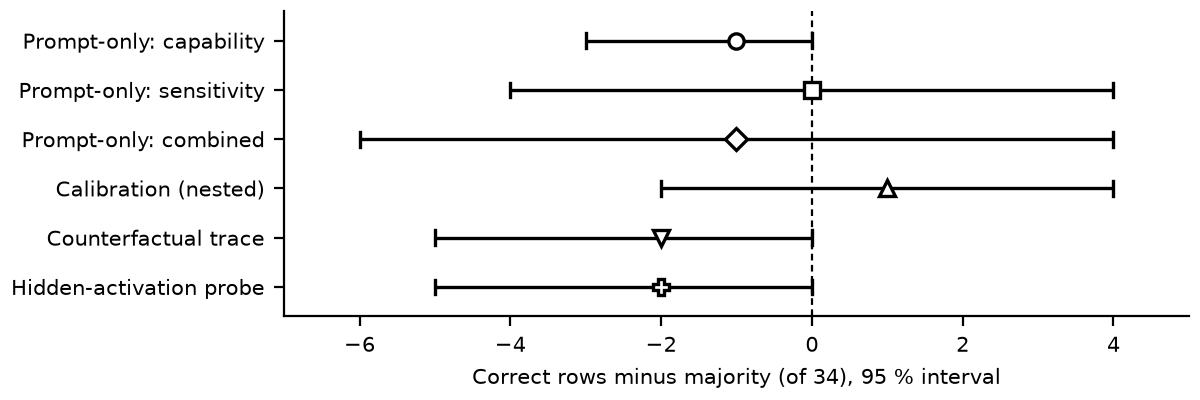
\includegraphics[width=0.85\linewidth]{forest.png}
\caption{Correct rows minus the majority baseline, with 95 \% problem-bootstrap intervals (Section 4 table).}
\end{figure}

Post hoc (Appendix B.2), no signal's held-out AUC interval lies above 0.5; calibration's is
0.67 {[}0.45, 0.95{]}, and at a prior-matched threshold it gets 24/34, the majority's count.

\begin{itemize}
\tightlist
\item
  \textbf{Generation stability} (12 labelled rows, no gate): largest Spearman with \texttt{max\_drop} 0.24
  (p = 0.46); the best of 13 leave-one-out rules, chosen after the fact, gets 9/12 against 8/12.
\item
  \textbf{Forced-answer flips:} 52/86 against a majority of 51/86 (Lesson 8).
\end{itemize}

\section{What we learned}

\begin{enumerate}
\def\labelenumi{\arabic{enumi}.}
\tightlist
\item
  \textbf{Sensitivity of a fixed trace is not sensitivity of the answer.} The answer-changing control
  moved the likelihood more in 33 of 42 traced configurations, yet the contrast did not separate labels.
\item
  \textbf{The label is about perturbations of solved problems, and nearly every row is solved.} In the
  organisers' two DeepSeek sets, 52 of 54 and 138 of 141 rows have base accuracy 1.0, and 79 \% and
  74 \% of those are non-robust (Lesson 6).
\item
  \textbf{Forcing the final answer does not rescue the answer-level test.} Held out, the flip rule gets
  18 of 34 train-file rows against a majority of 24, and its AUC is 0.71 on the train file and 0.40 on the organisers' set (difference 0.30 {[}\textminus{}0.01, 0.54{]}, not significant and confounded with model; Lesson 8).
\item
  \textbf{Robustness behaves like a property of the problem} (Lesson 9). Holding out one row instead of
  the whole problem lets a same-problem lookup gain 4 of 34 rows (one problem) and 8 of 43 (three
  problems) over the majority, balanced accuracy +0.20 {[}0, 0.40{]} and +0.33 {[}0, 0.46{]}; the length,
  prompt-only and calibration fits gain at most two rows there, so the strict split does not explain
  their nulls (Appendix B.3).
\end{enumerate}

\textbf{For the next entrant.} Hold out whole problems (a row-split lookup gains up to 8 of 43 rows);
report balanced accuracy (labels 71 \% robust, public sets about half); check the public sample
against the training file (5 of its 10 problems carry labels); report a text-length control; give
answer-level signals more than 4,096 tokens (10 of 12 Qwen3.5-4B rows gave no final answer within 8,192 tokens, Appendix B.2; Lesson 7 reports a check whose outputs were not kept).

\textbf{A text-length control.} On the organisers' 141-row DeepSeek set (137 problems), a logistic
regression on four counts of the problem text (log characters, words, digits, \texttt{\$}) reaches balanced
accuracy 0.644 (0.592 to 0.677 over 20 seeds) under five-fold problem-grouped folds; the 95th
percentile of its label-shuffle null is 0.592. The kit's uncertainty-profiling README reports 0.626
on the same rows with its own folds (its accuracy, 0.6879, is 97 of 141), so the comparison is
indicative. Log character count alone reaches 0.698; always answering non-robust has accuracy 0.745. Run once on our 10 DeepSeek rows, that artifact gets 2 of 10, too few to measure (Appendix C).

\section{Reproduction}

Code, saved features and commands: the supplementary ZIP (the same files, with the authors' names, are in a public repository whose link went to the organisers for the compliance check and is withheld here for anonymous review), \texttt{supplementary.zip} with \texttt{MANIFEST.sha256}, under Apache-2.0. \texttt{REPRODUCE.md} recomputes
Sections 1 to 4 on a CPU in about seven minutes on two CPU threads from the saved features and the data files of Appendix D. The scored
entries are the v3 uploads of 2026-10-27, a per-configuration prior fitted on the training file alone whose posteriors all
exceed 0.5, so both answer ``robust'' for every problem, the decision these results support (Appendix A). Our v1 entries of 2026-10-19 picked the configurations to call robust from ten single-configuration public-board
uploads, which is public-board feedback; we raised this with the organisers on 2026-10-24 and replaced them.

\section*{Related work}

Our signals follow work on a model's own reliability: self-evaluation (Kadavath et al., 2022), semantic
entropy (Kuhn, Gal and Farquhar, 2023) and hidden-state probes (Azaria and Mitchell, 2023; Burns et al.,
2023); our perturbations follow Shi et al.~(2023) and Mirzadeh et al.~(2024). Written chain-of-thought
can misreport what drove an answer (Turpin et al., 2023; Lanham et al., 2023), so our trace signal scores
how a fixed prefix responds to edits. Rows from one subject inflate predictions in small samples (Kapoor
and Narayanan, 2023; Rosenblatt et al., 2024); our repeated problems are such subjects.

\section*{Limitations}

Generation stability (12 rows) and forced-answer flips (86 rows) were scored on their own row sets,
not in the Section 4 table. The 34-row sample gives about 20 independent problems. Local models
are a proxy for the official deployments (Lesson 4). No white-box ablation was run, so the entry makes no White-Box claim. The Olmo-3-7B-Think forced-answer run was stopped (Appendix B.1). No signal was tested across model families without shared problems, and neither the main track nor the public sample was scored with any of the six signals. Calibration's interval on 34 rows leaves a true gain of up to four rows (12 points) unexcluded. We built no extra labels, although the organisers allowed them from 19 September.

\section*{AI Use Statement}

In this work, we used generative AI tools for ideation, coding, analysis and writing. Claude (Anthropic, through Claude Code) proposed methods, wrote the code, ran the experiments and analyses and drafted this report; OpenAI Codex (through the Codex CLI) helped plan experiment rounds and reviewed code and claims. We did not use generative AI tools to create or change any label (all labels are the organisers'), to decide which entries were uploaded to Codabench, or to submit this report. We have reviewed all AI-assisted work and take full responsibility for the final content of this report, including AI-assisted text, claims, code and other artifacts. Every number was rerun from the scripts named in this report, except Lesson 7 (36 of 36 samples without a final answer), whose outputs were not kept, the Olmo progress count read from its log, and the Codabench scores, IDs and board ranks of Appendices A and D, which were read from the competition pages and our submission log and have no script.

\section*{References}

\begin{itemize}
\tightlist
\item
  Azaria, A., Mitchell, T. (2023). The Internal State of an LLM Knows When It's Lying. Findings of
  EMNLP 2023.
\item
  Burns, C., Ye, H., Klein, D., Steinhardt, J. (2023). Discovering Latent Knowledge in Language
  Models Without Supervision. ICLR 2023.
\item
  Kadavath, S., et al.~(2022). Language Models (Mostly) Know What They Know. arXiv:2207.05221.
\item
  Kapoor, S., Narayanan, A. (2023). Leakage and the Reproducibility Crisis in Machine-Learning-Based
  Science. Patterns, doi:10.1016/j.patter.2023.100804.
\item
  Kuhn, L., Gal, Y., Farquhar, S. (2023). Semantic Uncertainty: Linguistic Invariances for
  Uncertainty Estimation in Natural Language Generation. ICLR 2023.
\item
  Lanham, T., et al.~(2023). Measuring Faithfulness in Chain-of-Thought Reasoning.
  arXiv:2307.13702.
\item
  Mirzadeh, I., et al.~(2024). GSM-Symbolic: Understanding the Limitations of Mathematical
  Reasoning in Large Language Models. arXiv:2410.05229.
\item
  Rosenblatt, M., et al.~(2024). Data Leakage Inflates Prediction Performance in Connectome-Based
  Machine Learning Models. Nature Communications, doi:10.1038/s41467-024-46150-w.
\item
  Shi, F., et al.~(2023). Large Language Models Can Be Easily Distracted by Irrelevant Context.
  ICML 2023.
\item
  Turpin, M., Michael, J., Perez, E., Bowman, S. R. (2023). Language Models Don't Always Say What
  They Think: Unfaithful Explanations in Chain-of-Thought Prompting. NeurIPS 2023, arXiv:2305.04388.
\item
  AIMO Interpretability Challenge organisers. getting-started kit,
  github.com/aimo-interp/getting-started, commit \texttt{de79405}.
\end{itemize}

\appendix
\section{Submission history}

Every upload to the competition, in order. Hashes are of the zips in the
lane's \texttt{dist/}, all of which the archive ships (\texttt{dist/entry/}, \texttt{dist/probe/}, and the two constant baselines); full hashes are in \texttt{REPRODUCE.md}.

\begin{center}
\footnotesize\setlength{\tabcolsep}{4pt}
\begin{tabular}{@{}p{3.3cm}p{2.6cm}p{1.7cm}p{0.9cm}R{1.3cm}p{1.9cm}@{}}
\toprule
File & sha256 (first 16) & Uploaded & Task & Id & Public score \\
\midrule
\texttt{always-true-main.zip} & \texttt{ba38cb0e7b55dd3a} & 2026-10-11 & main & 977178 & 0.48 \\
\texttt{always-true-small.zip} & \texttt{a3748c648a5a0d9a} & 2026-10-11 & small & 977183 & not recorded \\
ten single-configuration probes, \texttt{probe/*.zip} (nine zips kept) & see \texttt{REPRODUCE.md} & 2026-10-18 & both & not recorded & main best 0.57, small best 0.57 \\
\texttt{main-hybrid-v1.zip} & \texttt{d2df7dc8a0daaf85} & 2026-10-19 & main & 1002314 & 0.57 \\
\texttt{small-groups-v1.zip} & \texttt{82344d44e9b9d86e} & 2026-10-19 & small & 1002316 & 0.64 \\
\texttt{small-hybrid-v1.zip} & \texttt{376c170a05b963c8} & 2026-10-19 & small & 1002317 & 0.57 \\
\texttt{main-training-v3.zip} & \texttt{c315e32fc6392fb3} & 2026-10-27 & main & 1014009 & 0.48 \\
\texttt{small-training-v3.zip} & \texttt{470ceba57ca85278} & 2026-10-27 & small & 1014010 & 0.50 \\
\bottomrule
\end{tabular}
\end{center}

The two constant baselines answer ``robust'' for every configuration. Our submission log notes that the
first \texttt{always-true-small} upload had gone to the main task and was rejected at ingestion, so
its small-task score is not recorded; the log counts the small public set as 7 of 14 robust (0.50).

The probes each answered ``robust'' for one model configuration and non-robust for the rest. Their
net robust counts on the public sets (score times problems, minus the all-non-robust score) were,
main: Qwen3.5-4B 0, Olmo-3-7B-Think 0, DeepSeek-R1-0528-Qwen3-8B -1, gpt-oss-120b low -1,
gpt-oss-120b medium +1 (0.57), Skywork pending (cancelled); small: Qwen3.5-4B +1 (0.57), Skywork -1,
Olmo -1, DeepSeek +1. The small-track DeepSeek +1 is derived from the log's total, not a measured
score. The log lists the main-track DeepSeek probe as -1 on 2026-10-18 and as cancelled on 2026-10-19;
the public board holds five scored main-track probe rows from 2026-10-18 whose nets (0, 0, -1, -1, +1)
match the five values above, but which id is which probe was not recorded. \texttt{small-hybrid-v1} scored
0.57 (8 of 14; public board, read 2026-10-27). The public sets are 21 main and 14 small problems, so counts of +/-1 are
noise-sized, as the log notes itself; the v1 groups were chosen by those counts and can be
overfit to the public sets. \texttt{small-groups-v1} answers ``robust'' for Qwen3.5-4B and DeepSeek
(public 9/14 = 0.64, the sum of the two probes' counts, one of them derived). \texttt{main-hybrid-v1} answers ``robust'' for
gpt-oss-120b at medium effort only. Both hybrids replace DeepSeek's answer by the prediction of the
organisers' bundled uncertainty-profiling artifact (\texttt{uncertainty\_profile/}, run on DeepSeek's own
greedy trace); the small hybrid also keeps Qwen3.5-4B robust. That artifact is not one of the six
signals tested above; scored afterwards on 10 of our rows, it got 2 against a majority of 7 (Section 5). On the public main set the hybrid scored
0.57, the same as the gpt-oss-medium probe alone. None of these v1 entries uses a signal that
cleared its gate; they used public-board feedback and are withdrawn. The v3 entries use no public-set signal: their prior is fitted on the organisers' training file alone. Guarded v2 hybrids (\texttt{entry/}, built by \texttt{entry/build.sh})
were built and not uploaded.

\subsection*{Submission bundle (v3 training-only entries)}

Each zip holds a \texttt{solution.py} and \texttt{training-prior.json}; the small-track zip also holds the root-level
\texttt{small.txt} marker the competition requires there and forbids in a main-track one (kit README). There
is no artifact and the code reads no clock. \path{entry/fit_training_prior.py} fits a beta-binomial prior
(strength 64, chosen by leave-one-problem-out log loss inside the training data) on the 2026-10-15
training file (94 rows, sha256 \texttt{e18eb442\ldots{}}) and writes \texttt{entry/training-prior.json}. A configuration with
at least five labelled rows takes its posterior robust rate, any other configuration the track's global
rate, and a rate of 0.5 or more answers ``robust'' for every problem of that configuration:

\begin{center}
\small
\begin{tabular}{@{}lp{3.0cm}R{2.9cm}R{2.0cm}p{2.4cm}@{}}
\toprule
Track & zip sha256 (first 16) & Training rows & Global posterior & Answers \\
\midrule
main & \texttt{c315e32fc6392fb3} & 37 (gpt-oss-120b only) & 0.757 & ``robust'' everywhere \\
small & \texttt{470ceba57ca85278} & 43 & 0.721 & ``robust'' everywhere \\
\bottomrule
\end{tabular}
\end{center}

Every configuration's posterior is at least 0.5, so both entries make the same predictions as the
constant baselines; a configuration missing from the training file takes the global rate. The prior
is refitted with \path{entry/fit_training_prior.py} (command in REPRODUCE.md section 6). The v2 hybrids
were built and not uploaded. \texttt{entry/build.sh\ v3} fixes the file timestamps and the file
order, so two builds give the same bytes (\texttt{entry/test\_entry\_v3.py}, line 175).

\section{Methods, results and gates in full}

\subsection{Gates}\label{sec:B1}

The gates are in the table in Section 3. Commit and result times: prompt-only \texttt{8821dd5} 2026-10-11
14:36, results 17:49; calibration \texttt{7ba8061} 2026-10-11 19:53, results 21:22; trace \texttt{8f7abe9}
2026-10-13 12:04, rows 14:16; activation \texttt{2c49bc8} 2026-10-14 11:16, result 14:50; flips \texttt{6303f85}
2026-10-14 15:10, rows file 15:10.

``Set before it ran'' rests on git commit times against file times of untracked, unsigned run files,
and holds only for the prompt, calibration, trace and activation gates. For the first flips run it
cannot be shown: its rows file is stamped 25 s before the gate's commit (the gate line is
unchanged since). That run was unforced and gave no result: DeepSeek-R1-0528-Qwen3-8B produced no
final answer within 4,096 tokens on 36 of 36 samples (Lesson 7), and it was stopped. The reported
52/86 run came three days later with the final answer forced. Its Olmo-3-7B-Think job was stopped at
24 of 108 prompts (\path{runs/force-r4/Olmo-3-7B-Think.log}), so no Olmo row enters the flip test; Olmo
has 9 labelled rows. Calibration's control of 23 was the
prompt probe's own result, already known when its gate was committed.

\textbf{Prevalence.} A count that beats a 71 \%-robust majority says little about a near-balanced private
set, so the table reports balanced accuracy (any constant answer scores 0.500). The trace and
hidden-activation gates also required balanced accuracy of at least 0.70; those two probes reached
0.458, and no nested-selection result in the table exceeds 0.579 (the descriptive arm in B.2 reaches 0.60). \texttt{report/balanced\_gates.py} prints these values from
the saved reports. The forced-answer test saved no held-out predictions; its majority class is
non-robust (rows are 40.7 \% robust), and it was 52/86 against 51/86.

\subsection{Results}\label{sec:B2}

\begin{itemize}
\item
  \textbf{Prompt-only features:} capability features 23/34 (balanced 0.479), sensitivity 24/34 (0.558),
  combined 23/34 (0.567). The gate needed at least three more correct than majority; the margin
  was -1, and -2 after dropping the worst problem group.
\item
  \textbf{Calibration:} 25/34 (0.735, balanced 0.579) under nested problem holdout, one more than
  majority; the family holdout fell to 22/34 (balanced 0.604). The family holdout is not a
  held-out-problem test: the problems in the held-out family appear in training under the other
  models, and Lesson 9 shows their labels are nearly identical across models. The leak favours the
  method, and the figure still does not beat the majority of 24. The descriptive arm
  ability + difficulty + sensitivity, fitted as a fixed arm, reached 26/34 (balanced 0.60) and was
  chosen in 12 of 20 outer folds, but the pre-set nested selection gave 25/34.
\item
  \textbf{Post hoc ranking} (not part of any gate; \texttt{report/posthoc\_auc.py}, \texttt{report/posthoc\_auc.json}).
  For each gated signal except forced-answer flips, the held-out score behind the table's
  prediction (same model, same training rows, same inner selection; each score cut at the model's own
  threshold reproduces the reported correct count). AUC has robust as positive, with a 95 \% interval
  from 10,000 resamples of whole problems. The prior-matched cut predicts robust for the highest
  scores so that the predicted share equals the mean training-fold robust share (0.706, 24 of 34
  rows); ties at the cut all count as robust.

\begin{center}
\small
\begin{tabular}{@{}p{4.2cm}p{2.6cm}R{2.2cm}R{2.0cm}@{}}
\toprule
Signal & Held-out AUC, 95 \% interval & Correct / 34 at the prior-matched cut & Correct / 34 reported \\
\midrule
Prompt-only: capability & 0.43 {[}0.14, 0.89{]} & 22 & 23 \\
  Prompt-only: sensitivity & 0.57 {[}0.36, 0.82{]} & 18 & 24 \\
  Prompt-only: combined & 0.59 {[}0.32, 0.93{]} & 22 & 23 \\
  Calibration (nested selection) & 0.67 {[}0.45, 0.95{]} & 24 & 25 \\
  Counterfactual trace sensitivity & 0.39 {[}0.14, 0.64{]} & 20 & 22 \\
  Hidden-activation probe & 0.35 {[}0.17, 0.66{]} & 18 & 22 \\
\bottomrule
\end{tabular}
\end{center}

  Every interval includes 0.5. The pooled cut mixes scores from different folds, so it is
  descriptive only; the always-``robust'' majority gets 24/34.
\item
  \textbf{Generation stability:} on the 12 labelled Qwen3.5-4B rows, the largest rank correlation of
  any stability statistic with \texttt{max\_drop} is Spearman 0.24 (p = 0.46, 12 rows; change in mean log-probability
  under the distractor; the 14 rows including the two unlabelled give 0.30, p = 0.30). The best leave-one-out threshold rule gets 9/12 (change in log-probability
  under typos, a different feature, the best of 13 chosen after the fact) against a majority of 8/12. In 10 of the 12 rows none of the four original samples
  reached a final answer within the 8,192-token cap, and the other two had one of four unanswered,
  so the agreement statistics are nearly constant. This signal had no predeclared gate.
\item
  \textbf{Counterfactual trace sensitivity:} the pilot traced 37 configurations, the 34 labelled ones
  and 3 from the unlabelled band; the 43-row refit appended 12 Skywork rows, so
  \texttt{runs/trace-pilot/rows.jsonl} now holds 49. Of the 34 labelled rows the probe is scored on, 31 had two or
  more verified variant families and 29 had the negative control; rows with a missing family or
  control enter with imputed values and a missing indicator. The probe reached 22/34 (balanced
  0.458), wrong on two rows the majority gets right and right on none it gets wrong; the family
  holdout reached 24/34, equal to its majority; the same leak applies to it.
\item
  \textbf{Refit on 43 rows} (2026-10-15 file; \texttt{report/intervals-43.json}, \texttt{report/posthoc\_auc-43.json}).
  Gates fail again: prompt-only margin \textminus{}2; calibration out-of-fold accuracy 0.698, net \textminus{}1 against
  the majority, one row above its control (30 against 29 correct); trace and hidden-activation probes do not
  pass. Balanced accuracy: 0.484, 0.477, 0.544 (prompt-only), 0.484 (calibration), 0.509 (trace),
  0.468 (activation). Post hoc AUC {[}95 \%{]}: capability 0.468 {[}0.16, 0.87{]}, sensitivity 0.570
  {[}0.34, 0.81{]}, combined 0.629 {[}0.34, 0.93{]}, calibration 0.460 {[}0.22, 0.76{]}, trace 0.513 {[}0.35, 0.69{]}.
\end{itemize}

\subsection{Row split and data snapshot}\label{sec:B3}

\textbf{Row split against problem split} (\texttt{report/split\_audit.py}; \texttt{report/split-audit.json} for the 34
pinned rows, \texttt{report/split-audit-1015.json} for the 43 rows of the newer file). Split A holds out one
(model, problem) row and keeps that problem's other rows in training; split B holds out the whole
problem, as every headline result does. Features, train-only preprocessing and arms were fixed
before the run. The same-problem lookup predicts a row from the training rows with the same problem
text, else the fold majority; it demonstrates the leak and is not a method. Intervals come from
10,000 whole-problem bootstrap draws (seed 0), both splits rescored on each draw.

\begin{center}
\small
\begin{tabular}{@{}p{2.8cm}p{1.9cm}p{1.9cm}p{2.2cm}p{2.4cm}@{}}
\toprule
Arm & 34 rows: correct A / B & balanced A \textminus{} B & 43 rows: correct A / B & balanced A \textminus{} B \\
\midrule
Majority & 24 / 24 & 0 & 31 / 31 & 0 \\
Four length features & 24 / 24 & 0 & 31 / 31 & 0 \\
Prompt-only combined & 23 / 23 & 0 & 31 / 29 & +0.03 {[}0, 0.07{]} \\
Calibration (nested) & 26 / 25 & +0.05 {[}0, 0.10{]} & 29 / 30 & \textminus{}0.02 {[}\textminus{}0.05, 0{]} \\
Same-problem lookup & 28 / 24 & +0.20 {[}0, 0.40{]} & 39 / 31 & +0.33 {[}0, 0.46{]} \\
\bottomrule
\end{tabular}
\end{center}

Under split A, 23 of 34 and 32 of 43 test rows have their problem in training. The lookup never
loses a row to the majority; every gain is a non-robust row, from one problem (34 rows) and three
problems (43 rows), so the lower bound sits at zero: a resample is positive whenever it draws one of those
problems, 1 \textminus{} (19/20)\^{}20 = 64 \% of draws on 34 rows and 1 \textminus{} (19/22)\^{}22 = 96 \% on 43, and none is negative. On 34 rows the length and prompt-only predictions are identical under both splits.
Calibration under split A keeps its inner search unchanged, which still holds out whole problems.
A label shuffle within each model, which keeps every model's robust rate, expects 3.9 agreeing
problems against 11 observed (34-row snapshot, all labelled models) and 4.9 against 11 on the small
track of the newer file; the pooled shuffle expects 3.8 and 4.7, and no shuffle of 2,000 reaches
the observed count in either. Model prevalence does not explain the agreement of Lesson 9.

The table keeps the 82-row snapshot of \texttt{train-main-v2} (pinned revision \texttt{23791d9b}), because gates
and features were frozen on it before the 2026-10-15 file existed. The newer file (94 rows) has 49
small-track rows, 43 of them labelled, over 22 problems, 31 robust; the 43-row refit uses it.

\subsection{Method details}\label{sec:B4}

\textbf{Prompt-only features.} One forward pass of the original prompt and of two surface
perturbations (typos, an irrelevant distractor sentence): prompt NLL and length, the change in NLL
under each perturbation, and the cosine change of hidden states at 50 \% and 75 \% depth. A
logistic probe over these eight features.

\textbf{Ability and difficulty calibration.} A per-model ability term and a per-problem difficulty term
estimated from prompt statistics, with covariates offered as arms (ability; +difficulty;
+covariates; +sensitivity) and the arm chosen inside the outer folds by inner leave-one-problem-out.

\textbf{Generation stability.} Qwen3.5-4B sampled on the originals and perturbed prompts; agreement and
accuracy drop between them, compared with the labels' \texttt{max\_drop}.

\textbf{Counterfactual trace sensitivity.} A deterministic 256-token reasoning prefix is generated from
the original prompt. It is then teacher-forced after the original prompt and after verified
answer-preserving variants: variable renaming (with the rename applied inside the trace),
equivalent numeric expressions, equation-side swaps and reordering of independent givens. A
condition change that alters the answer (one integer constant raised by one) is the negative
control. Eleven predeclared features: the prefix's mean log-probability under the original prompt, the
per-token log-likelihood change (mean, worst family,
variance, concentration in the least likely 20 \% of tokens), hidden-state cosine change at 50 \%
and 75 \% depth (also near renamed entities), the ratio of answer-preserving to answer-changing
sensitivity, and indicators for missing families and a missing control. Only trace positions are
captured, and activations are released per problem.

\section{Lessons in full}

\begin{enumerate}
\def\labelenumi{\arabic{enumi}.}
\item
  \textbf{The sample is smaller than it looks.} 34 rows from 20 problems give about 20 independent
  units. The Section 4 intervals are 3 to 10 configurations wide, so a real gain of one or two
  configurations could not be seen here.
\item
  \textbf{Prompt features did not beat the majority.} Capability features reached 23/34, sensitivity
  24/34 and the combined arm 23/34 against a majority of 24 (Section 4). One possible reason is that
  the label is a difference between two accuracies and a feature of one prompt sees only one side
  of it; we did not test this.
\item
  \textbf{Sensitivity of a fixed trace is not sensitivity of the answer.} The trace features measure a
  likelihood response, not whether the final answer survives the perturbation: teacher-forcing
  one reasoning prefix under a renamed or reordered problem measures surprise at the edit. The control that changes the answer moved the likelihood more in 33 of the 42
  traced configurations that have one (49 traced, 7 without a control; median ratio of
  answer-preserving to answer-changing change 0.62; on the 29 labelled rows with a control, 22 of
  29, median 0.62; \texttt{report/trace\_control.py}), so the features see the edits; the contrast still did not separate the labels.
\item
  \textbf{Local models are a proxy for the official deployments.} Qwen3.5-4B ran in BF16; Olmo-3-7B-Think,
  DeepSeek-R1-0528-Qwen3-8B and Skywork-OR1-Math-7B ran in 4-bit NF4. Neither matches the
  organisers' serving setup, and the NF4 rows may carry quantisation effects in the trace
  features. We report this as a limitation, not as an explanation of the null result.
\item
  \textbf{Hidden states did not help either.} A linear ridge probe on each model's native hidden
  states (prompt and a 128-token reasoning prefix, pooled at 25, 50 and 75 \% depth, families kept
  in separate coordinates) reached 22/34 under the same nested problem holdout, two below the
  majority (\texttt{fit\_activation\_probe.py}, \texttt{run\_activation\_probe.py}).
\item
  \textbf{The label is about perturbations of solved problems.} In the organisers' augmented sets,
  problems whose every base sample was correct are still mostly non-robust. The two sets are the
  same model, DeepSeek-R1-0528-Qwen3-8B (the kit's \path{uncertainty_profile/config.py} maps the id
  \texttt{qwen3-8b:low} to it), and all 52 problems of \texttt{augmented-sample-math-agg-filtered} also appear in
  \texttt{augmented-sample-math-agg} (137 problems), so the two figures are not two models. Rows are per permutation type, so a problem can appear in several rows: the filtered set has
  54 rows over 52 unique \texttt{problem\_id}, the larger set 141 rows over 137. Rows with \texttt{base\_accuracy}
  = 1.0 (any number of base samples, 1 to 60) are 52 of 54 and 138 of 141, nearly all rows, so the
  non-robust share among them (41 of 52, 79 \%; 102 of 138, 74 \%) matches the unconditional share
  (43 of 54, 80 \%; 105 of 141, 74 \%). Restricted to rows with exactly ten base samples: 34 of 40
  (85 \%) and 63 of 82 (77 \%). \texttt{report/lesson6\_counts.py} computes all of these. Answer consistency
  on the original cannot be tested in these sets. The public evaluation sets are near balance
  (always ``robust'' scores 0.48 on the main task, and the small-model set is 7 of 14 robust) while our 34
  labelled rows are 71 \% robust (Section 1), so a majority vote learned on the training rows is
  not a safe default.
\item
  \textbf{Answer-level tests run out of token budget.} We started an answer-flip test (each model
  answers the original, typo and distractor copies, and a renamed copy where the problem has a name). DeepSeek-R1-0528-Qwen3-8B
  produced no final answer within 4,096 tokens on 36 of 36 samples of the olympiad problems. This
  check is not reproducible from the archive: its outputs were not kept. We did not run the
  unforced test further; Lesson 8 forces the final answer instead.
\item
  \textbf{Forcing the final answer does not rescue the answer-level test.} We reran the answer-flip
  test with the final answer forced: each unfinished sample is continued from its reasoning with
  \texttt{\textless{}/think\textgreater{}} and \texttt{The\ final\ answer\ is\ \textbackslash{}boxed\{} appended, greedy, 24 tokens. Rows: the
  2026-10-15 \texttt{train-main-v2} small-track labels (Qwen3.5-4B 12, Skywork-OR1-Math-7B 12,
  DeepSeek-R1-0528-Qwen3-8B 10; 34 rows, 24 robust) plus the 52 DeepSeek rows of the organisers'
  aggregated set \texttt{augmented-sample-math-agg-filtered} (11 robust); four samples per variant at
  2,048 tokens, Skywork and DeepSeek with FP8 weights. Under the same problem-held-out protocol
  the best rule reached 52/86 against a majority of 51/86, short of the gate. This rule is fitted on all 86 rows; refitted per source it gets 59, against 65 for a majority taken per source.

  The sign of the signal differs between the two row sets, and the data do not tell label source
  from model apart: the two sets share no model except DeepSeek, and the DeepSeek train-file rows
  alone are 10 rows. \texttt{report/flips\_by\_source.py} joins the rows to their source and prints, for
  the AUC of the mean flip rate (above 0.5 means robust rows flip less) with a 95 \% interval from
  4,000 bootstrap resamples of problem ids (seed 0):

\begin{center}
\small
\begin{tabular}{@{}p{3.6cm}R{1.4cm}p{1.2cm}p{1.7cm}R{2.8cm}@{}}
\toprule
Label source & Rows (robust) & Mean-flip AUC & 95 \% interval & Problem-held-out rule, correct / majority \\
\midrule
2026-10-15 train file, Qwen3.5-4B & 12 (8) & 0.703 & & \\
  2026-10-15 train file, Skywork-OR1-Math-7B & 12 (9) & 0.685 & & \\
  2026-10-15 train file, DeepSeek-R1-0528-Qwen3-8B & 10 (7) & 0.738 & {[}0.12, 1.00{]} & \\
  2026-10-15 train file, all & 34 (24) & 0.706 & {[}0.44, 0.87{]} & 18 / 24 \\
  Organisers' per-permutation set, DeepSeek & 52 (11) & 0.402 & {[}0.22, 0.59{]} & 41 / 41 \\
\bottomrule
\end{tabular}
\end{center}

  The difference, train file all minus organisers' set, is 0.304 {[}\textminus{}0.01, 0.54{]}.

  The train file labels a model on a problem by the largest accuracy drop over the perturbation
  families (Section 2). In the organisers' \texttt{augmented-sample-math-agg-filtered} (54 rows),
  \texttt{permutation\_type} is a single type for 43 rows (32 \texttt{domain}, 59 \% of all 54) and a list for 11
  rows (3 one-element \texttt{{[}"distract"{]}}, 8 with two to five types). All 34 \texttt{domain} and \texttt{rephrase} rows are non-robust, so the 11 robust rows are among the other 20,
  while our typo, distractor and rename copies include neither permutation. Restricted to the 12 rows
  whose problem has only typos, distract or rename permutations in every one of its source rows (8 single-type rows, 4 list rows; 4
  robust), the mean-flip AUC is 0.547 {[}0.10, 0.89{]} (same 4,000-draw problem bootstrap,
  \texttt{-\/-permutations}). With fewer than 5 robust rows the restricted test is underpowered and cannot say
  whether the sign reverses. The earlier pooled
  DeepSeek figure (0.348 on 62 rows) mixed both sources. On the competition-style labels the
  in-sample AUC is 0.71, but the held-out rule gets 18 of 34 against a majority of 24, so the
  null stands. The 52 augmented rows give 41 against 41, again no gain.
\item
  \textbf{Robustness behaves like a property of the problem, which makes public scores easy to
  inflate.} \texttt{report/lesson9\_counts.py} computes these counts from the organisers' parquet files, and \texttt{report/lesson9\_shuffle.py} the shuffle null.
  \texttt{train-main-v2} labels 33 problems. At the pinned revision (82 rows, \texttt{23791d9b}), 11 of them are
  labelled for more than one model and all 11 carry the same label for every model; counting
  each reasoning effort of gpt-oss-120b as its own configuration, 15 problems are labelled for
  more than one configuration and 14 of those agree. In the 2026-10-15 file used for the
  forced-answer test (94 rows), the figures are 14 of 33 with 13 agreeing by model, and 16 with
  15 agreeing by configuration. The rule that any model counts as a repeat is the loose one; the counts are small
  either way. On the small track alone the shuffle expects 4.7 agreeing problems (range 2 to 7).
  The one disagreement mixes a Skywork row with gpt-oss-120b rows, so it crosses tracks. Five of the ten problems in the public challenge sample appear in \texttt{train-main-v2}
  with labels (same count in both files). A lookup over labelled problems can therefore score
  well on public problems that overlap the training labels; we did not measure it on unseen private
  problems, and we read public scores far above the majority with that overlap in mind. Appendix B.3
  measures the same lookup on our labels under a row split and a shuffle that keeps each model's
  robust rate.
\end{enumerate}

\textbf{The organisers' artifact, scored once on our labels.} The uncertainty-profiling example is not
one of the six signals; both v1 hybrids shipped it (Appendix A); the v3 entries ship no artifact. \texttt{report/artifact\_gate.py} generated
greedily with DeepSeek-R1-0528-Qwen3-8B on the 10 DeepSeek rows of the 2026-10-15 train file (10
problems, 7 robust; 4,096 new tokens; the kit's pinned library versions; most layers offloaded to the
CPU on a 12 GB card, which changes speed, and greedy tokens only through floating-point differences)
and applied the artifact's estimator and decision threshold unchanged (\path{runs/artifact-gate/score.json}).
It scores 2/10 against a majority of 7/10: balanced accuracy 0.333, difference \textminus{}5 rows with a 95 \%
whole-problem bootstrap interval of {[}\textminus{}10, 0{]}. It predicts non-robust for 9 of 10 rows; both correct
calls are non-robust rows, and the probability that a robust row scores below a non-robust one is
0.14. Ten rows with three non-robust cannot measure its accuracy. They are consistent with a
threshold set where 74.5 \% of rows are non-robust and applied to labels that are 70 \% robust.

Its README documents a grouped out-of-fold balanced accuracy of 0.6262 and plain accuracy 0.6879
(\path{kit/solutions/uncertainty-profiling/README.md}, lines 127-128; DeepSeek only, on the organisers'
aggregated set). That is below this report's own 0.70 balanced bar, so by our standard it would not
clear a gate either. A constant ``non-robust'' scores 105/141 = 0.745 on that set, above the
artifact's 97/141. Our ten rows count against it, and the v2 bundles that use it were not entered.

A length baseline (\texttt{report/length\_baseline.py}) tests the 0.626 against problem length. On the
same 141 rows (137 problems), five-fold problem-grouped folds, seeds 0 to 19, a standardized
logistic regression with balanced class weights on four features of the problem text (log
character count, word count, digit count, \texttt{\$} count) reaches balanced accuracy 0.644 (0.592 to
0.677) and accuracy 0.664; log character count alone reaches 0.698 (accuracy 0.702). A
label-shuffle null (200 shuffles that permute labels across problems, rows of one problem kept
together, one seed each) has median 0.498, 95th percentile 0.592 and maximum 0.647. The
artifact's 0.6262 is not shown to beat problem length; its own folds and threshold differ from
these, so the comparison is indicative.

Transfer to the organisers' public sample (\texttt{report/sample\_transfer.py}): labelling the 558-row sample by the proposal paper's outline, which the organisers say differs from the official rule
(largest \texttt{absolute\_accuracy\_decay} per model and problem, robust at most 0.10, non-robust from 0.25), gives 69 labelled
(model, problem) pairs of 80 over 10 problems, 38 robust. Five of the 10 problems are also in \texttt{train-main-v2}, and only
\texttt{gpt-oss-120b:low} and \texttt{qwen3-8b:low} (taken to be DeepSeek-R1-0528-Qwen3-8B) match a training configuration; the per-configuration prior
predicts robust for both, so it scores 8 of 15 labelled pairs, the same as the pooled majority. The pooled per-problem arm needs
features that do not exist for these problems (a GPU run), so it was not tested there.

\section{Reproduction details}

Code, saved features and exact commands: the supplementary ZIP (the same files, with the authors' names, are in a public repository whose link went to the organisers for the compliance check and is withheld here for anonymous review), \texttt{supplementary.zip} with \texttt{MANIFEST.sha256}, released under Apache-2.0 (\texttt{LICENSE} in the tree).
\texttt{REPRODUCE.md} recomputes the numbers in Sections 1 to 4 on a CPU in about seven minutes on two CPU threads from the
saved features and the data files below, and lists the data file, script and run folder behind each section; regenerating the
hidden-activation features needs a GPU. Data, all Hugging Face datasets of the organisation \texttt{aimo-interp}, none redistributed:

\begin{itemize}
\tightlist
\item
  \texttt{aimo-interp/train-main-v2} at revision \texttt{23791d9b120132087877\allowbreak{}b0459f953d5959fc8455},
  \path{data/train-00000-of-00001.parquet}, sha256 \texttt{bedfb551ea0f4d95d5e70e1df7cf6139\allowbreak{}5ce2d36eeba2869aba6a90fc3c198824}.
\item
  \texttt{aimo-interp/train-main-v2} as of 2026-10-15 (\path{data/train-main-v2/train-2026-10-15.parquet}, 94
  rows), sha256 \texttt{e18eb44207e7987781ec2ff214793196\allowbreak{}038442bdc1466fdf5498f3e87ec58285}. At revision
\texttt{fa8af758c6519fc97a9d\allowbreak{}0bd9017feb6f12232b52}, downloaded 2026-10-17.
\item
  \path{aimo-interp/aimo-interp-challenge-sample-full} (the public sample of Lesson 9),
  \texttt{validation-00000-of-00001.parquet}, sha256 \texttt{2989ab6a018f2779a821209f414bd004\allowbreak{}9c9ef1c2488f589ff2d3bf4ed16942ff}.
  File dated 2026-10-11 in the data folder; no revision recorded.
\item
  \path{aimo-interp/augmented-sample-math-agg} (Lesson 6), \texttt{validation-00000-of-00001.parquet}, sha256
  \texttt{b785750259a3f4524cbaf988f5166019\allowbreak{}7cbdfca19d8f45cc35347d4ef29aa4db}. The organisers' kit pins
  revision \texttt{f972ced0705096f8d7ca\allowbreak{}7fac30825900b8b7fb6a}; we did not record the revision of our
  copy (file dated 2026-10-11), so the match is not verified.
\item
  \path{aimo-interp/augmented-sample-math-agg-filtered} (Lessons 6 and 8), same file name, sha256
  \texttt{b8a485868ce5a14d0c961e009e30bc61\allowbreak{}f850ad2d2224a01ae1ada401fb73ed3d}. File dated 2026-10-11 in
  the data folder; no revision recorded.
  Training
  code: this repository (\texttt{fit\_probe.py}, \texttt{sub/calibration.py}, \texttt{fit\_trace\_probe.py},
  \texttt{fit\_activation\_probe.py}). Organisers' kit: \path{github.com/aimo-interp/getting-started} at commit
  \texttt{de79405}. Competition: https://www.codabench.org/competitions/16180/.
\end{itemize}

The v1 uploads, replaced by the v3 entries on 2026-10-27, and their scores (Appendix A; board position on 2026-10-19): \texttt{small-groups-v1}
(static groups, no artifact) scored 0.64; \texttt{main-hybrid-v1} scored
0.57; \texttt{small-hybrid-v1} scored 0.57. The hybrids run the organisers' artifact for DeepSeek; none of the three uses a signal tested here. The v2 bundles were built and not
uploaded. Codabench IDs of the v1 uploads are in Appendix A. The leaderboard lists eight probe rows, IDs 1000868, 1000873, 1000876, 1000878, 1000884, 1000887, 1000891 and 1000892; \texttt{REPRODUCE.md} lists the zip hashes of the nine kept. Appendix A
describes the shipped v3 bundle (main id 1014009, score 0.48; small id 1014010, score 0.50).
\end{document}
